

\documentclass[notitlepage]{report}
\usepackage[left=1in, right=1in, top=1in, bottom=1in]{geometry}
\usepackage{graphicx}
\usepackage{titling}
\usepackage{lipsum}
\usepackage{amsmath}
\usepackage{svg}
\usepackage{float}

\pretitle{\begin{center}\Huge\bfseries}
\posttitle{\par\end{center}\vskip 0.5em}
\preauthor{\begin{center}\Large\ttfamily}
\postauthor{\end{center}}
\predate{\par\large\centering}
\postdate{\par}

\title{The Lightlane Argument}
\author{Gelanor Rhadamantys}
\date{\today}
\begin{document}

\maketitle
\thispagestyle{empty}

\begin{abstract}
Metaphysics are axiomatic system that 



"Deep Quantum Theories", and summarize a selection of them. Common ground is identified, and a representative theory called Deep Quantum Automaton is presented.


\end{abstract}

\section*{Introduction}
After 100 years of quantum mechanics, the formalism is essentially proven. Through countless experiments, the predictive strength is verified beyond a sliver of a fraction of the smallest possible doubt (Planck doubt $D_P$). Let there by no doubt, Quantum Mechanics works and is the most true theory of reality humanity has ever possessed. However, almost as illustrious as the successes of the theory in predicting physical phenomena, is the failure to anchor the theory in a metaphysical framework. This has been an issue from the very beginning of QM. But, at the start of the previous century, it was important to the founders of the theory to direct focus on the theory and its predictive power itself, and not the confusing and "inappropriate" way that the theory worked. In its infancy, the desire to intuitively understand QM theory through a classical lens was seen a threat to the survival of the theory itself. The disagreement between Bohr and Einstein was, at its core, precisely this. Einstein famously expressed his dislike for Bohrs Copenhagen Interpretation and D'Brogiles (TODO). He eventually came around once the experimental predictions were spectacularly verified. This marked a turning point, and the prevailing sentiment became to follow the theory, develop it and eventually an intuitive explanation would fall into place once the theory was fully explored.
After more 100 years, the theory has been explored and verified beyond any doubt. The theory however, is still seen as weird and counter-intuitive. This has led to a very peculiar situation : The theory is now being taught as something that cannot be intuitively understood, it's weirdness and it's quirkiness is treated as an orthodoxy that should not be challenged. It's something that a well behaved student of quantum mechanics simply must accept. Obviously, this is not satisfactory to everyone, and many great scientists have expressed their dissatisfaction in the same way as Einstein, separating their use of the theory on one hand, and in their spare time, dug into possible frames that could explain Quantum Mechanics in other, more salient ways.

I have been deeply enthralled by idea that a metaphysical foundation for quantum mechanics must exist, and I have held this belief for many years.  Attending conferences, reading and peering into the depths of the internet, I have found many like minded, and perhaps you are one. There are tens if not hundreds of attempts to anchor precisely this weirdness of the quantum in a metaphysical system that is less weird. As we shall see, some of them have been quite successful at explaining the weirdness of the Quantum World in novel ways. However, there has not been any definitive way to bring these metaphysical systems to the test. Humbly, I propose that I might have found a way to do.

In this paper I will begin by a meta-analysis of some metaphysical foundations of Quantum Mechanics, attempting to pinpoint their common ground. Finally, I will propose an "argument" that seems to be able to bring some of these metaphysical frameworks into the realm of observational experiments. The argument I propose is actually a constraint on the behavior of light, that translate into physical, measurable effects. The argument is  simply that a certain class of metaphysical system  impose this constraint on reality, in order for the metaphysical frameworks to remain free from self-contradictions. If the predictions that follow from this constraint is observationally verified, we have been able to bring metaphysical systems to the test for the first time. It is this constraint and its applications that enable us to connect the metaphysical to the physical that is possibly novel. The subsequent papers "Lightlane equality" and "Initial Lightlane predictions" and  "The Lightlane blur predicition" are simply technical investigations into the consequences of this argument. Finally, in the latest installment "The Equivalence of Implementation" seeks to bring these consequences into an even more profound, and perhaps useful conclusion.


\section*{Deep Quantum Theories}
To do this, we must first qualify what we mean by "metaphysical system".  First, I must point out that metaphysical frameworks are not the same as physical theories. Instead of making predictions, frameworks exist purely to satisfy the human inclination toward beauty. Why we have expended so much energy looking into the dephts is an important question in it's own right. Why exactly do we have this preference, desire even, for seeking out a frame of thinking that are simpler, more elegant. Why is that such a powerful drive, and why do we associate this quest to understand with beauty? To be clear, there is no guarantee that whatever lies beyond quantum mechanics is simpler. It might be even worse, even more confusing, strange and alien than quantum mechanics itself. And yet, there is the case of Occams Razor. A principle that proclaims that if a simpler, more elegant explanation is possible, then this is probably the correct one. This tool, which requires us to expend a lot of energy simplifying has been instrumental in most, if not all of scientific discovery since the dawn of civilization. It is from this desire to simplify, understand and grasp that metaphysical systems emerge, and include religions, mythological systems and stories that help people make sense of the reality that surround them. 

But we need to be a bit more selective than that. We are interested in metaphysical systems that are able to explain Quantum Mechanics in ways that elicit a feeling of beauty, simplicity and completeness. We are interested in systems that naturally give rise to complexity and variabilit yet constrain this complexity in ways that are in accordance with Quantum Mechanics. We name these metaphysical system "Deep Quantum Theories".   Deep Quantum theories can be defined as "the class of theories that seek to explain Quantum Mechanics by means of a deeper, more profound mechanism". As such, all Deep Quantum theories attempt to bridge the intuitive gap between natural philosophy and quantum mechanics, but might be starting from different starting points. Some starts from a philosophical starting point, and reasons onward from first-principles. Other attempt to work backwards, starting with elements of Quantum Mechanics and see to explain these features through alternate, deeper mechanics.

However, it is important to discern this class of Deep Quantum theories from Quantum Theory reformulations. Loop Quantum Gravity for example, is not a Deep Quantum Theory, but a fully equivalent Quantum Theory. It is an attempt to reformulate Quantum Mechanics using a different set of building blocks. However, theories like Loop Quantum Gravity remain important because they might act as crucial stepping stones for Deep Quantum theories to make contact with real physics.

This longing for a more intuitively understandable theory is not a new thing, and has roots in the evolution of Quantum Mechanics itself. For example, Schrödinger coined the term $Zitterbewegung$, or trembling-motion to explain in more intuitive terms the phenomena of quantum indeterminacy required by Quantum Mechanics. Another system we will review, is  T'Hoofts model of Cellular Automata. This is able to show a connection between the behavior of periodic patterns in Cellular Automata (CA) and QM. In that the quantum mechanics is a statistic over an extremely fast, extremely high resolution, but fully deterministic underlying reality. A third interpretation is Tegmarks Mathematical universe. In this proposal, reality is mathematical. Within this complex web of mathematical relations, enough complexity emerge  that the relationships themselves constitute matter. When this mathematical matter organizes itself in such a configuration that it becomes sentient, that is - develop consciousness, this consciousness has no choice but to  observe these mathematical structures from within. It is even possible that all these metaphysical systems are simply different ways of expressing the same thing: That reality is a subset of something much bigger, such as the set of information structures that allow a consciousness to emerge, powerful enough to ponder the answer to the question of life, the universe and everything. I will make brief pause here to let that sink in. 

Now! I just wrote the words "mathematical universe watching itself from within". This will not do. We need to get our feet back on the ground. There are important quantum phenomena that we need to address, but before we can do that we need to explain briefly what they are.


\section*{Quantum Indeterminancy}
Quantum Mechanics requires that particles exhibit a rather surprising "either/or" behavior.  For example, a quantum particle can be either in an up state or a down state,  but never in between. This is called superposition, usually given as "the particle exists in an undefined state of both up and down at the same time". But how can something be both up and down at the same time? We could try to formulate a more understandable explanation, such that the particle is actually rotating, but that there are only some positions that can be detected. However, there is another feature of this behaviour which is puzzling. We shall call it quantum "stuckness". After a measurement has been made telling us that the particle was "up", the particle gets stuck in this particular state for a while. If the particle was rotating, then this could indicate that the measurement stopped the rotation. But that doesn't make any sense either, because if we leave it alone for a while - it will start "rotating" again.  In that case, where did the energy from the rotation go, and where did it come from when it started again. What I am trying to illustrate here is that rotation, our first metaphysical explanation for the quantum either/or behaviour is not very satisfying. But what we can glean from this though exercise is the following:

Our metaphysical system must explain all of the following:
\begin{enumerate}
\item Superposition: Why the particle can be up and down at the same time, either because it is rotating or something else. 
\item Quantization: When we measure the particle, it becomes either the "up" state or the "down" state, and not anything in between.
\item Stuckness:  When we have measured the particle, it remains in the "up" or "down" state so that if we measure it again, we know beforehand what result we will obtain.
\end{enumerate}

\section*{Quantum Entanglement}
The second in our list of weird quantum behaviour we need to explain, is called Quantum Entanglement. Already we are at the core of the problem, because quantum entanglement is considered to be at the very  core of quantum weirdness. To explain this very briefly, whenever two quantum particles are brought into contact with each other, they become entangled. This means that they share probabilistic behaviour. For example, if two particles are entangled in a specific way, and then separate them - they are both in the superposition state. But because they have some kind of link, if you detect that the one is in the "up" state, you also know that the other is in the "down" state, simply because you know that they are entangled. It seems as the first particle is able to send a "message" to the other, telling it to be in the opposite state. The weirdness of this is that this is true instantaneously, no matter the distance. The particles could have been entanglend millions of years ago, and separated by millions of miles. Even so, with the equations of quantum mechanics, detecting that particle $A$ is in state up, we also know that particel $B$ is in state "down". If our metaphysical theory is that one particle is sending the other a message, then this message must travel faster than the speed of light.!If we allow information to travel faster than light, this makes the entire theory of relativity to fall apart. There simply must be another explanation for this quantum entanglement than messages being sent back and forth, and our Deep Quantum theory need to explain it.
What we can glean from this quantum phenomenon, is that our metaphysical Deep Quantum Theory must be able to explain the following:

\begin{enumerate}
\item Entanglement mechanism: When two particles come into contact with each other, they start to interact in a way that provides a mechanism for this shared behaviour. 
\item Instant knowledge : Knowing something about $A$ means you know something about $B$ instantaneously, no matter the distance.
\item  Speed limit : Whatever our Deep Quantum Theory cannot transmit information faster than the speed of light. 
\end{enumerate}

As you can plainly see, if you had not abandoned the idea of a spinning particle from the Quantum Indeterminancy already, you have no choice now. Our Deep Quantum Theory needs to be able to explain all these phenomena easily, beautifully and precisely or it cannot be what we are looking for.



\section*{Deep Quantum candidates}
We have now reviewed two important quantum phenomena, but there are several more tests to come. But this serves us well as a starting point. There are in fact several metaphysical systems that are able to handle most of these problems beautifully. 

\subsection*{Copenhagen interpretation}
First a word on the current mainstream interpretation, the Copenhagen Interpretation. Even if this is the most accepted interpretation, it is in many ways also the simplest to reject. It is mentioned here, because of its status as the most accepted interpretation, for it is not a Deep Quantum theory. In fact, it doesn't even attempt to explain the origin of the quantum weirdness. The Copenhagen interpretation is what you a get when you decide that spending time and energy trying to find an explanation for Quantum weirdness is unnecessary and therefore a waste of time. Proponents of this interpretation argue that we should not insist on a classical way to understand the universe. Quantum Mechanics has proven that the universe it not classical, so looking deeper, trying to resurrect a classical understanding of Quantum Mechanics i wrongheaded. They would argue that we don't need a Deep Quantum Theory, because Quantum Mechanics is the ultimate truth - there is no deeper level, so we don't need to look for it. This can be a very practical standpoint, allowing you to learn and use Quantum Mechanics studying other problems. Taken at face value however, the position is more economical than scientific - arguing that it's better to invest in understanding how to use the theory than explaining why it is the way it is. And they might be right, perhaps there is no deeper level that explains the weirdness in ways easier to understand. But the question remains, if  there are other theories capable of explaining the the theory in simpler, more beautiful terms, wouldn't we want to know? Wouldn't we still have Quantum Mechanics, and all the gifts that it has brought even if we could explain it better?


\subsection*{Bohm-De Brogile Pilot Wave theory}
One of the early attempts to challenge the Copenhagen interpretation was introduced by the jesuit priest Gilles De Brogile. At the famous Solway conference. 



\subsection*{Many worlds theories}





\subsection*{Cellular automata theories}




All these three branches of Deep Quantum theories have very different metaphysical foundations. The two first remain continous theories
The Quantum Indeterminacy is only one of several types of Quantum Weirdness that the metaphysical foundation must be able to account for. But we shall not bite over more than we can chew. The first requires that the act of detection affects the particle itself, triggering it to "collapse" into a definite state. The second is even weirder, suggesting that there are multiple possible realities going on at the same time, and unless we are able to separate them from each other, we experience both (all) at the same time.
The third suggest that the particle is - in fact - in a specific state any given time $t$, but that it transitions between the states so quickly that it is essentially random which we "pick". Once we measure it, it is forced to obtain one value and keep it for further experiments. Keep in mind, we are now looking only at indeterminacy and entanglement.

In addition to quantum indeterminancy, whatever explanation is the correct one must be consistent with Quantum Entanglement as well. 

TABLE : 						Bohm DeBrogile		 	Many Worlds	      	Digital
Indeterminancy					OK								OK						OK
Entanglement					FAIL								FAIL						OK
Repeat detections				Shaky							OK						Shaky
Speed limit						Shaky						     OK						OK


Several of the theories here explicitly require a grid-like information structure, onto which the deep quantum reality is operating. The existence of such a grid is hinted at by the success of quantum theories using a grid, such as Loop Quantum Gravity. For all the theories 
that have a grid-structure embedded in them, there are two  important questions: 

\begin{enumerate}
\item If you can express a quantum theory by means of a grid, does that make the grid real? Or can there be other reasons for this to work?
\item Is quantization as it appears in QM a fingerprint of this deep quantum theory, operating on a grid?
\end{enumerate}

There is no doubt that quantization is an important concept in QM. The question here is it's origin. If such fingerprints can be detected, we do more than increase our understanding of the universe, we can revolutionize the philosophical foundations of quantum mechanics. 

To see this argument, it's important to understand the significance of the Loop Quantum Gravity reformulation of Quantum Mechanics. A reformulation of an existing theory is a powerful move, because it suggests that all the successes of ordinary quantum theory could have been realized through the reformulated approach, had it been discovered first. As theories, they are in effect equal. The success in reformulating Quantum Mechanics by quantizing spacetime and realizing all particles as features of the information state suggest that if a Deep Quantum Theory exists, it is going to be grid-based. At the same time, the intuitive success of Grid Based Deep Quantum Theories to explain some of the counter-intuitive things that happen in Quantum Mechanics points toward the same target, but from a different direction.

\section*{Common foundations of Deep Quantum Theories}

\begin{enumerate}
\item Information based
\item Explain quantum entanglement
\item Quantum indeterminancy
\end{enumerate}


We wil's important to emphasize that theories which attempt to invalidate Quantum Mechanics does not fall into this group. All the theories mentioned in this paper clearly state that they believe quantum mechanics to be accurate. 

I will here briefly discuss a number of theories that all fall under the umbrella term "Deep Quantum Theories" and what they have in common. As previously mentioned, quantization is the key feature that unites these different intuitions. The theories also differ in what they focus on explaining.

\section*{Calculating space, Simulation hypothesis}
Describe the common foundations, illustrate using Cellular Automata.

\section*{Reality as mathematical relation }
Tegmark has written

\section*{Wheelers "It from bit", }
Describe the common foundations, illustrate using Cellular Automata.

\section*{Lazlo Biocentrism}
Describe the common foundations, illustrate using Cellular Automata.

\section*{Loop Quantum Gravity}
Loop Quantum Gravity uses a model where quantum interactions are understood as the interaction between open and closed loops, that move around on quantized positions on spacetime. It can be argued that Loop Quantum Gravity through this model of quantum fundamentals rests on an axiomatic foundation where everything is quantized, including the substrate of spacetime itself. This has important implications, because it implies that the Information Hypothesis is also part of the axiomatic foundation of Quantum mechanics. A consequence of this is that we implicitly cast every particle that exist as an information pattern encoded on this n-dimensional lattice. 
The space of possible  configurations of reality is inherently also quantized, governed by the number of orientations that the grid can support, the amount of information implicated etc. For example, the quantization of position, direction, speed, energy levels and momentum might be nothing more than tell tale signs of the quantizedness of spacetime itself. This quantised legacy might in turn leave fingerprints about the constraints these information system operate under in real world observations. 

\section{Elementary Cycles theory}
Donatello Dolce has conceived of a 
\section*{All is number}
The all is number theory is overlapping significantly with other Deep Quantum theories, but 

\section*{Are Deep Quantum theories falsifiable?}
Describe the common foundations, illustrate using Cellular Automata as a model. If such theories to be falsifiable, they need to either produce predictions that can be detected in the Quantum realm, or possibly even higher. 

\begin{enumerate}
	\item  The broad class of deep quantum mechanisms, provide specific predictions that only make sense. This is difficult because the Deep Quantum theory cannot really make predictions about anything, because it's internal workings remain unknown - if it even exists.
	\item  If a Deep Quantum theories are real, then Quantum Mechanic must be a probablistic model to approximate a deep quantum theory. This means that there might be restrictions on what a quantum theory can do,  due to it being a statistic over a deep quantum theory. This way, a deep quantum theory can be falsified by detecting phenomena that a deep quantum theory cannot possibly support.
	
\end{enumerate}
For the class of Deep Quantum theories we are concerned about, those DQT that are based on a Quantized foundation, the restriction must come from the fact that the deep quantum theory is quantized. 
	
\section*{Constraining the class further }
The class of Deep Quantum Theories are so far only defined by having a quantized foundation. It is however possible, to further subdivide such DQT into subclasses depending on their relation to Determinism. 

\begin{enumerate}
\item Deterministic, randomness only apparent
\item Non deterministic, allow randomness
\end{enumerate}

For the Deterministic Deep Quantum theories (DDQTs).  Tegmark and Wolfram fits within this framework.

\section*{Deterministic, pseudo-random }
It is known that Quantum Mechanics require randomness. if the QM is an probabilistic approximation of a DQA, then it is clear that a deterministic DQT must provide a source of randomnes that is indistinguishable from the randomness. 

\section*{Other sources for the randomness observed in nature }
In order to be able to follow an the Xyston argument, we are faced with a difficult choice. We can either introduce all the ideas at the same time, or we can postpone certain important questions to a later time. The first would be preferable, were it not for the complexity of the subject matter. I have tried,and failed, at introducing these ideas in parallel, but struggle with both my own and the readers cognitive bandwidth. The second approach is the only viable path. This is unfortunate, but necessary to avoid being overwhelmed. As we proceed with the fleshing out of our Deterministc Deep Quantum Automaton, what it can and cannot do, we will see that it has a deterministic nature  we know is contrary to what we have learned about indeterminacy, randomness etc in quantum mechanics. It can be tempting to disregard the entire Xyston argument because it takes this departure from Quantum Mechanics. However, I can assure you that the difficult questions of Quantum Mechanics such as observer effect, superposition, quantum entanglement and and wave particle-duality are not simply ignored or looked away from. Rather, these questions will be reintroduced when we have a firm understanding of the limitations of the Deterministic Deep Quantum automaton. This is similar to studying the path of a photon, whilst keeping in mind that the unobserved photon has a position described over the probabilistic path-integral, that is all possible paths that the photon could possibly take through space.

Therefore, we will first assume photons to be deterministic machines capable of propagation, interation with other patterns through information exchange. For this reason they have primarily a particle-like nature. However, due to their non-physical nature of information objects, we will later be able to connect their behavior to the Schrödinger wave-function once we introduce indeterminacy.

\begin{enumerate}
\item Local hidden variable information systems with a well-defined position in space 
\item Deterministic propagation path through grid, determined by a part of the information pattern.
\item Looping, that is returning to a previous configuration at regular intervals.
\item Exhibiting conservation of energy interacting with other patterns.
\end{enumerate}

\section*{Deep Quantum Automaton }
From this filtering, we have found a class of Deep Quantum theory that has sufficient constraints on it that it can be tested.

\begin{enumerate}
	\item  The many worlds interpretation offer an alternative intuition to quantum entanglement
	\item  Provides succint explanations to some of the strangest phenomenons in quantum mechanics
	\item  Wave particle duality, double slit experiment and quantum entanglement.
	\item  Xyston argument presents a way to make specific predictions about light behaviour under a specific interpretation of quantum mechanics.
	\item The interpretation requires many worlds (to explain entanglement, all quantum observer effects, double slit experiment), the information hypothesis and a local hidden variable theory of quantum mechanics.
	\item If the predictions are supported by data from telescopes, this is a strong indication that the many worlds hypthesis is correct, because a strong indication of a precision cap on the directional freedrom of light would suggest that quantum indeterminancy cannot be fundamental to information propagation

\end{enumerate}
\section*{Introduction}

An approach to Quantum Gravity has been to continue on the path pioneered by Max Planck, assuming the quantized nature of reality. A notable success in this field is the work by Carlo Rovelli and his team and the reformulation of Quantum Mechanics on a grid like subtrate in their Theory of Loop Quantum Gravity. A reformulation of an existing theory is a powerful move, because it suggests that all the successes of ordinary quantum theory could have been realized through such a grid and information based approach, had the time of discovery of these different formulations of the same underlying reality been reversed. The success in reformulating quantum mechanics by quantizing spacetime and implementing all particles as features of the information state of this grid might be revealing  a deeper, more fundamental question.

Loop Quantum Gravity uses a model where quantum interactions are understood as the interaction between open and closed loops, that move around on quantized positions on spacetime. It can be argued that Loop Quantum Gravity through this model of quantum fundamentals rests on an axiomatic foundation where everything is quantized, including the substrate of spacetime itself. This has important implications, because it implies that the Information Hypothesis is also part of the axiomatic foundation. A consequence of this is that we implicitly cast every particle that exist as an information pattern encoded on this n-dimensional lattice. 
The space of possible  configurations of reality is inherently also quantized, governed by the number of orientations that the grid can support, the amount of information implicated etc. For example, quantization of position, direction, speed, energy levels and momentum might be nothing more than tell tale signs of the quantizedness of spacetime itself. This quantised legacy might in turn leave fingerprints about the constraints these information system operate under in real world observations.  If such fingerprints can be detected, we do more than increase our understanding of the universe, we can revolutionize the philosophical foundations of quantum mechanics. To see this argument, it's important to understand the significance of the Loop Quantum Gravity reformulation of Quantum Mechanics.

\section{The hard question of quantum mechanics}

How can dynamics be possible without time?

How can time travel be mathematically possible?

How can the double slit experiment make sense?

How can we explain the delayed quantum eraser experiment ?

How can we explain the photoelectric effect?

How can we explain that the universe is so fine tuned for life?

How can we explain quantum entanglement?

As above so below


\section{Deterministic Evolutionary  Emergence Process (DERP)}
It isn't surprising that a reformulation of a theory is possible.  But each reformulation brings with it an unique axiomatic foundation. The benefit of reformulations is to simplify relationships and to explore various ways of expressing the theory through different axiomatic ground rules. With Loop Quantum Gravity, the axiomatic foundations are radically simplified, using only

\begin{enumerate}
	\item  Grid or lattice network (space-time)
	\item  Information (duality)
	\item  Evolution (process)
	\item  Emergence (survival from interactions)
	
\end{enumerate}
Patterns of information states are encoded by the means of binary logic (duality), which is predicated only on an abstract substrate, such as a grid  or a network. Time can be seen as the relationship between information states on this grid, which may be direction agnostic. But if the evolution leads to an increase in entropy, there is an overall direction of time allowing for the definition of an arrow of time. The remaining complexity of our reality can be seen as emergent phenomena from this information undergoing evolution, selection and interaction. This begs the question, why does a reformulation under such minimalist assumptions work?

There are two possible answers:

\begin{enumerate}
	\item The reformulation was possible due to the inherent flexibility on how to formalize any self-consistent algebra. Under this interpretation,  a grid is a sufficiently flexible system to implement any algebra, and the fact that it works on Quantum Mechanics does not necessarily imply anything about the true nature of our universe. 
	\item The phenomena of quantization observed in quantum mechanics, and by extension in the real world, is inherited from a reality where spacetime is quantized. Such a reality would conforms to the DERP axiomatic foundation. This has the potential for intuitively explaining why quantization occurs and take so many forms.
\end{enumerate}

It's obvious that discerning between these two possible answers would provide us with deep insights either way. But if the second answer is true, the consequences would far exceed the obvious - to elevate the Loop Quantum Gravity formulation of Quantum Mechanics to canonical status. It would reach much deeper, and open up opportunities to probing  quantum mechanics at a deeper level than particle physics, through an entirely new field studying the foundational interactions that give rise to the forces of the universe.
In this paper we intend to make a the first foray into this world of DERP Quantum Theory. 



%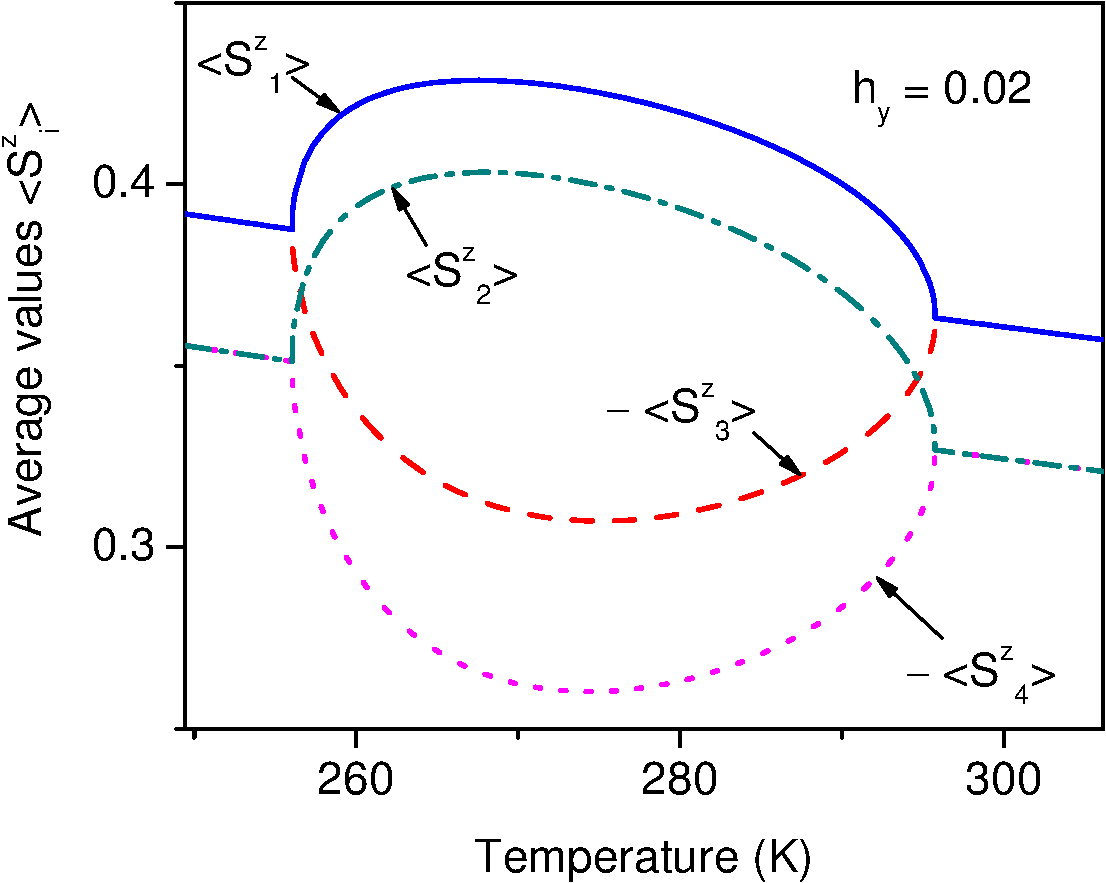
\includegraphics[width=0.65\textwidth]{eps_demo}
\end{document}
